This thesis project has involved the implementation and evaluation
of many different components required to create an end-to-end wheelchair
navigation assistance system.

\subsection{Evaluation of machine learning models on preliminary dataset}
%include speed
The YOLOv5, DeepLabv3, and Hybridnets models were tested on the preliminary
video-only Curtin driving dataset. As this dataset is unlabelled, the
models were evaluated in terms of speed and potential usage, rather than accuracy.

A frame of YOLOv5 evaluated on the preliminary dataset can be seen in \cref{fig:yolov5s}.
This model identifies vehicles and pedestrians with high accuracy, with the confidence in
a prediction decreasing as the object moves further away from the camera.

\begin{figure}[H]
    \centering
    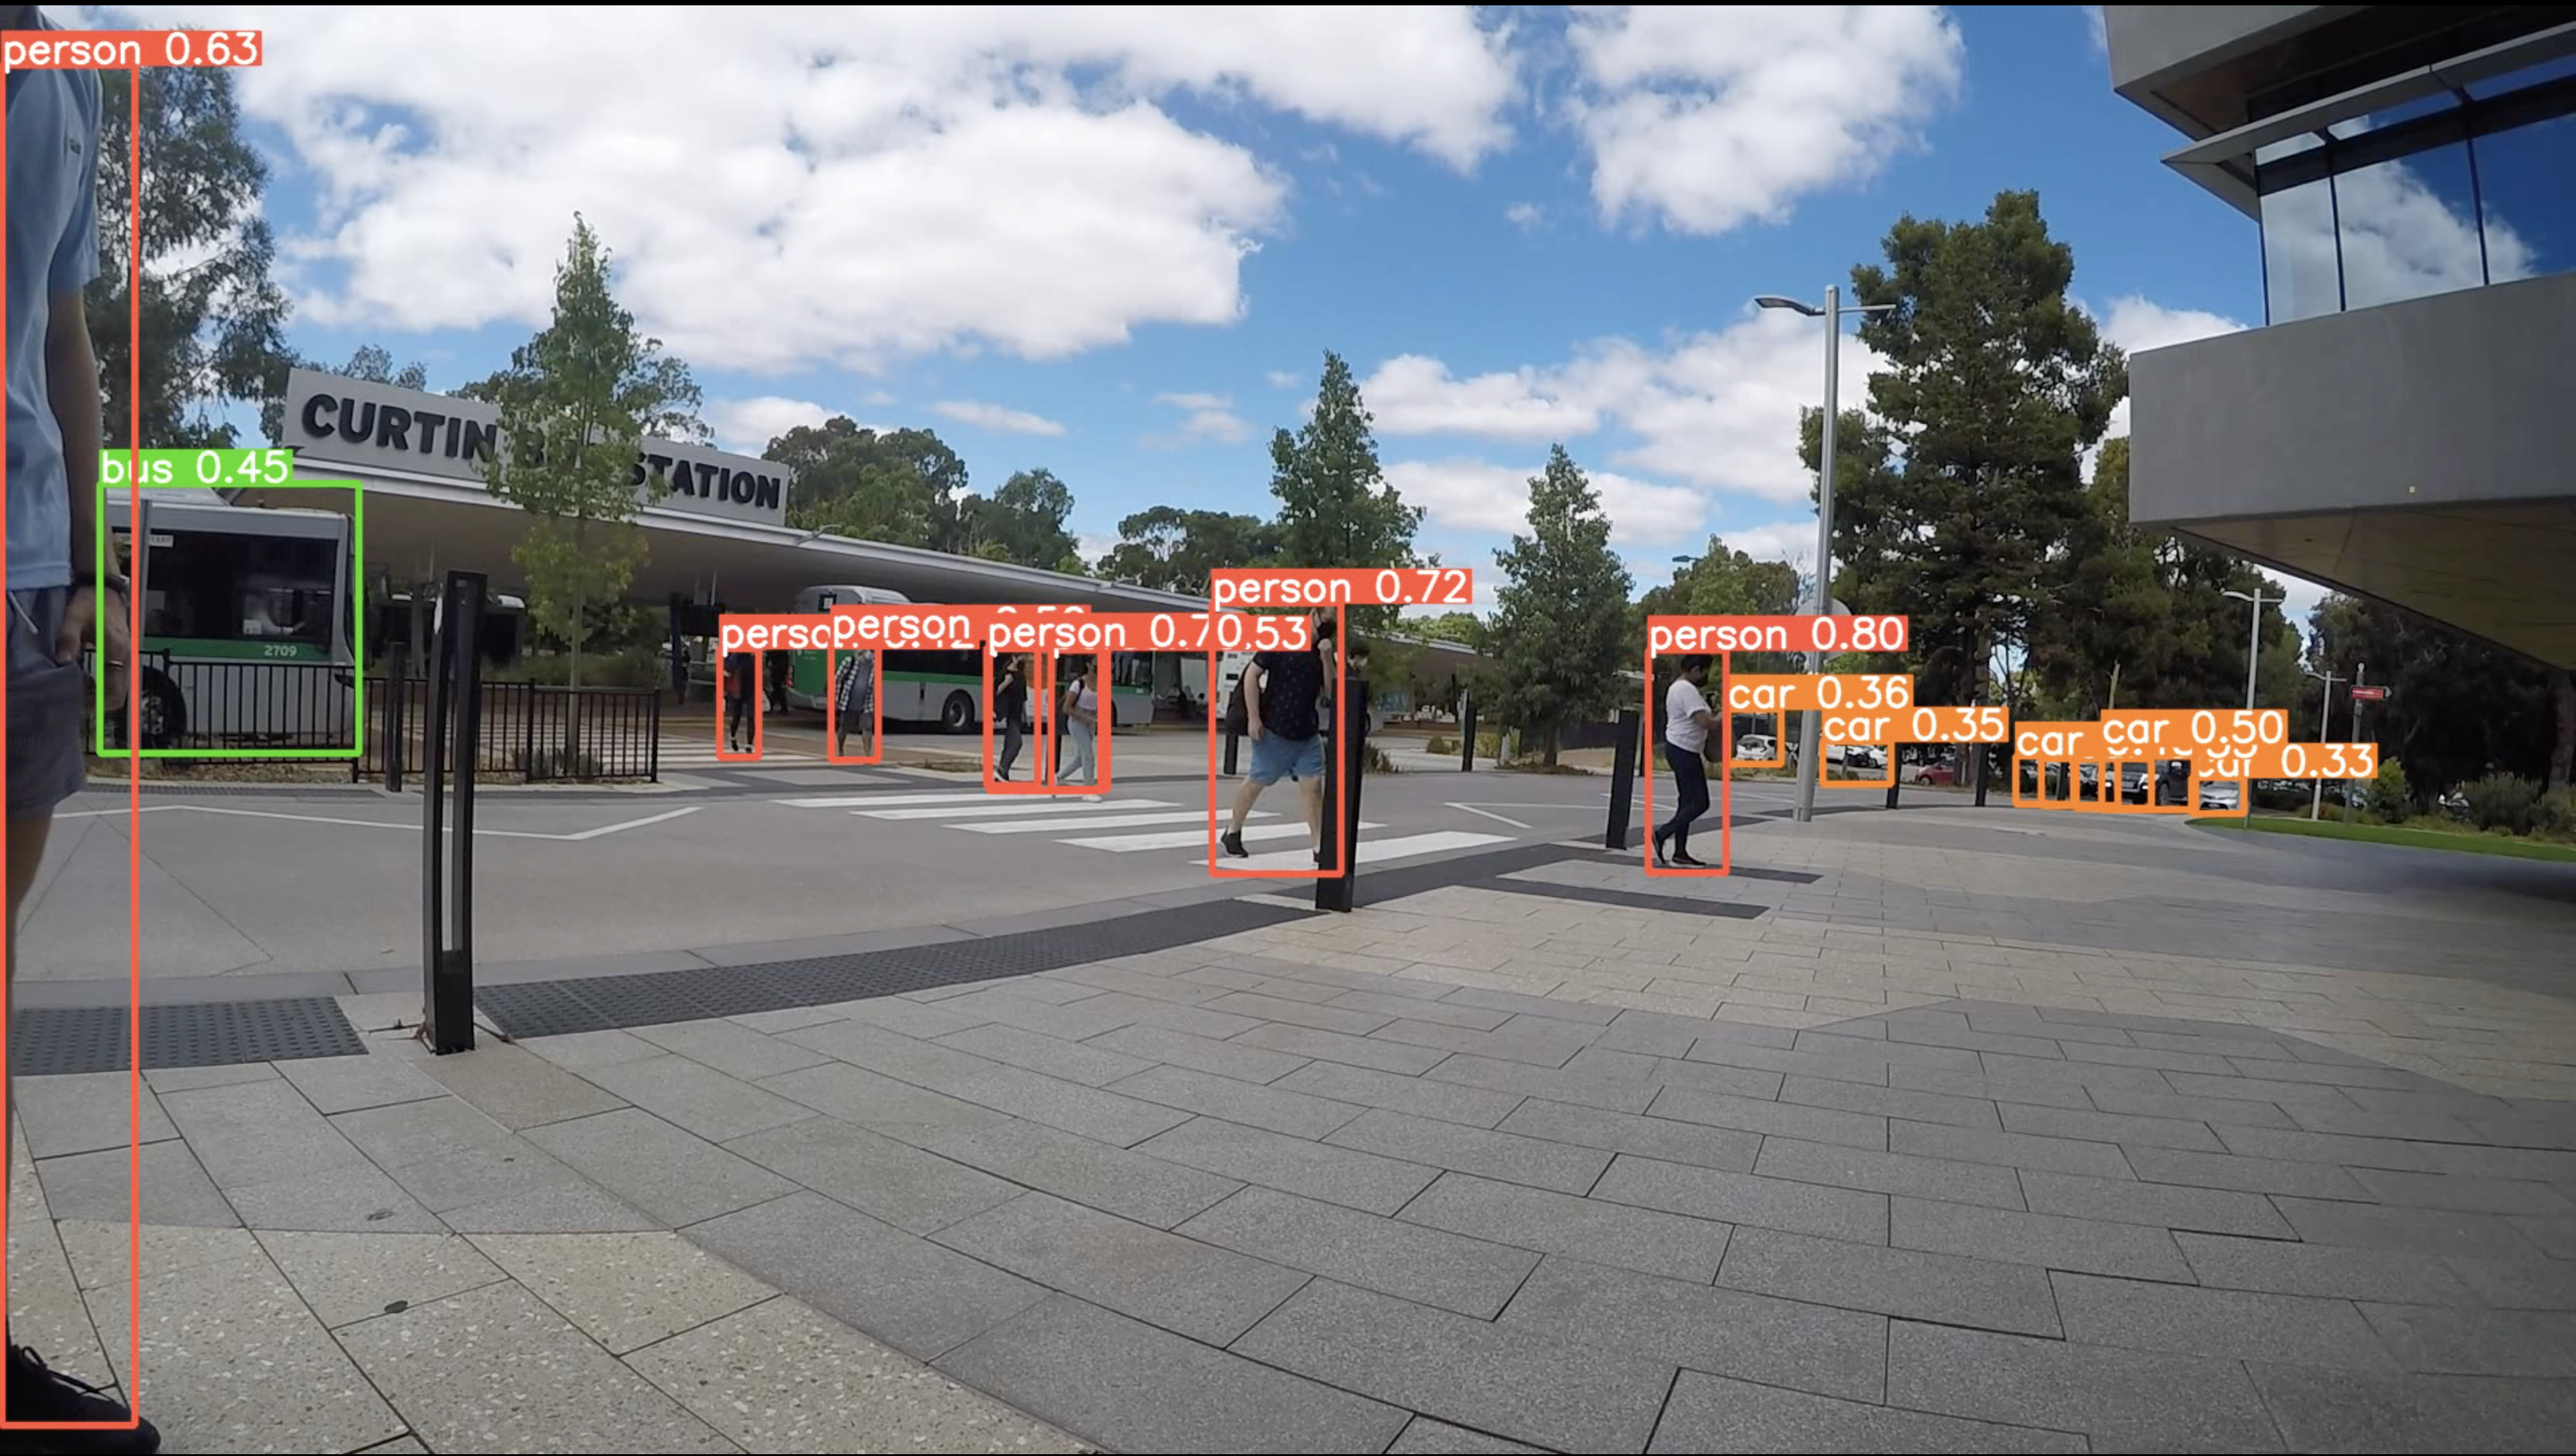
\includegraphics[width=0.65\linewidth]{images/yolov5s.png}
    \caption{YOLOv5s evaluated on the Curtin dataset}
    \label{fig:yolov5s}
\end{figure}

A frame of DeepLabv3 evaluated on the preliminary dataset can be seen in \cref{fig:yolov5s}.
DeepLabv3 identifies pedestrians with a high level of accuracy. However, the vehicles in the
image are not accurately segmented. This is likely due to the lower occurrence of vehicles
in the MS COCO dataset, which was used to train the model.
To repurpose this model for the task of drivable area segmentation,
it would have to be retrained on a labelled driving dataset such as BDD100K or Cityscapes.

\begin{figure}[H]
    \centering
    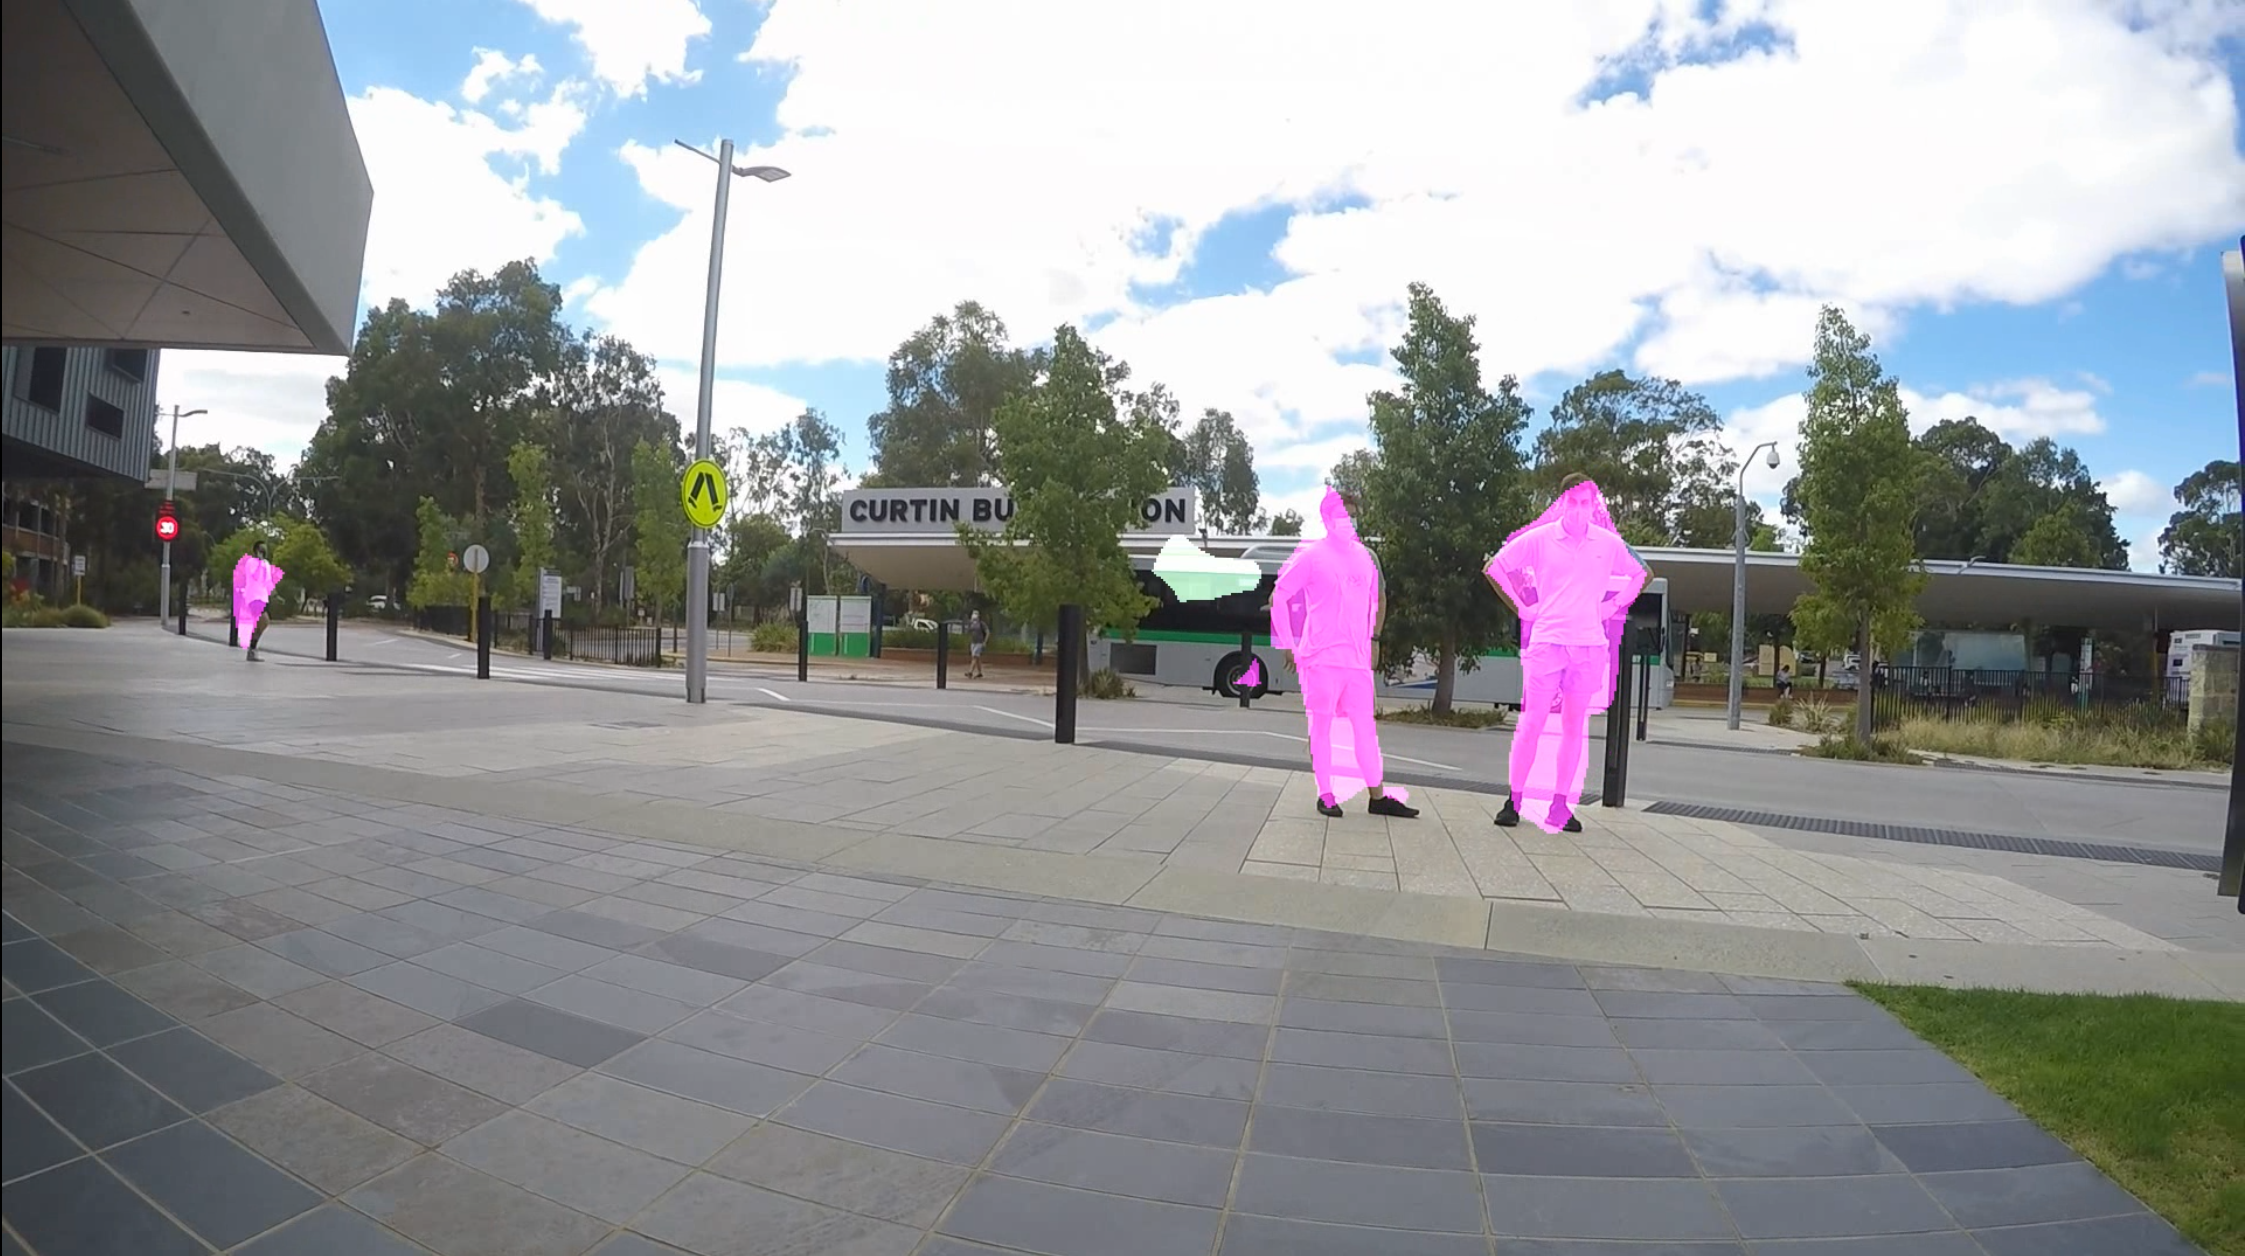
\includegraphics[width=0.65\linewidth]{images/deeplab.png}
    \caption{DeepLabv3 evaluated on the Curtin dataset}
    \label{fig:deeplab}
\end{figure}

An example of Hybridnets drivable area segmentation can be seen in \cref{fig:hybridnets}.
This model accurately detects drivable areas outdoors when a path is uniform, however
has more difficulty identifying a drivable path for non-uniform surfaces such as paved brick.
Hybridnets can also struggle to identify drivable paths indoors in some circumstances.
This is likely due to problems with domain adaptation, as the Hybridnets model was trained on the
BDD100K dataset which primarily consists of bitumen roads.
Hybridnets does not identify drivable area consistently when indoors
but does work well in some cases.

\begin{figure}[H]
    \centering
    \begin{subfigure}{.48\textwidth}
        \centering
        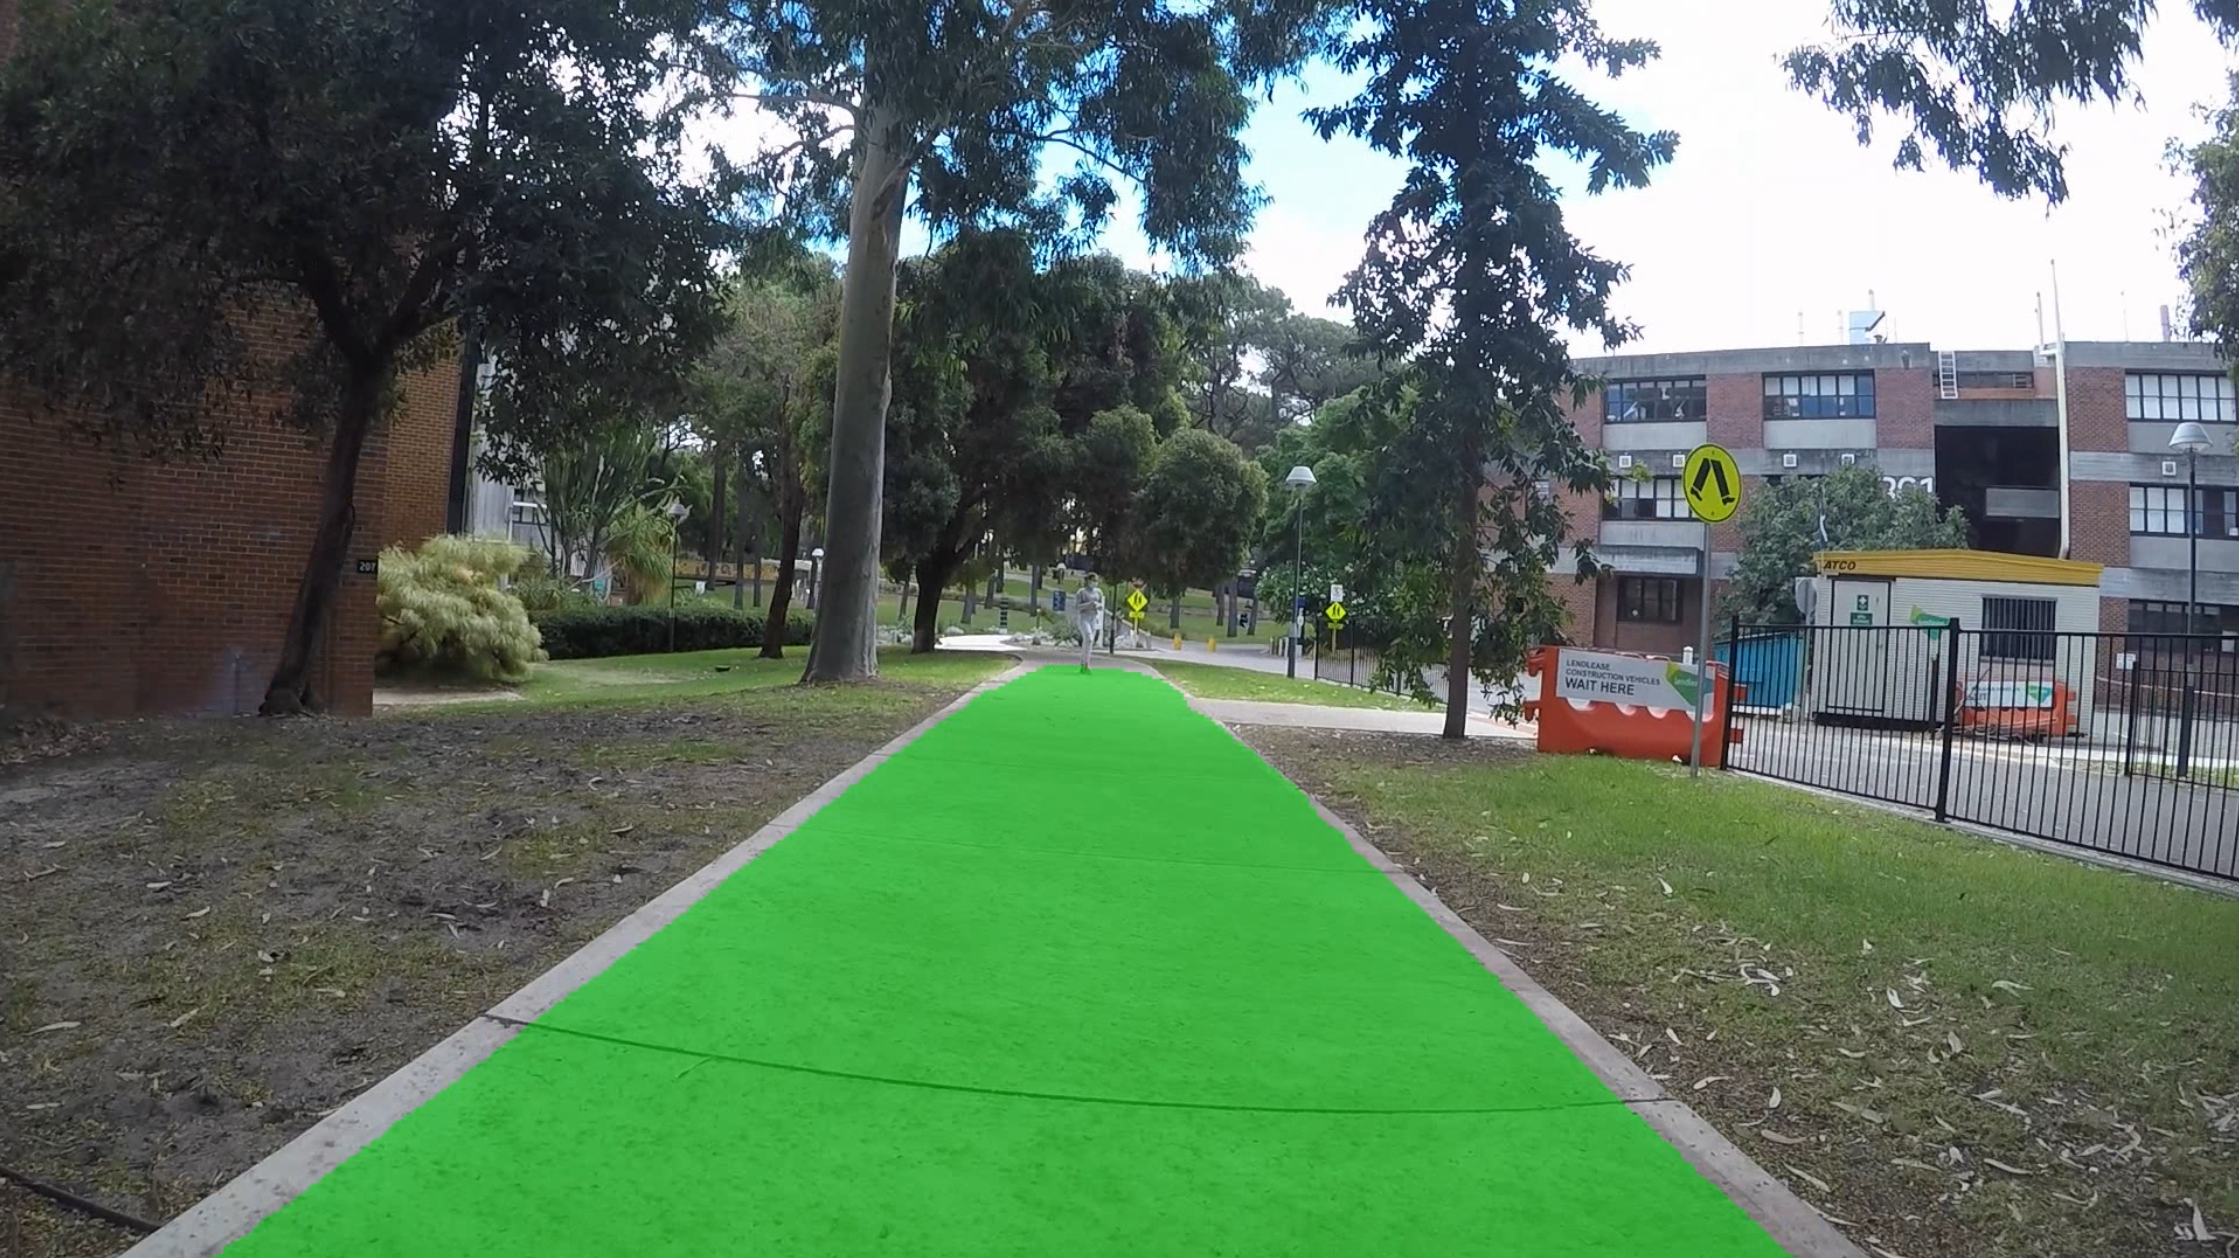
\includegraphics[width=\linewidth]{images/hybridnets_outdoor.png}
        \caption{Outdoors}
    \end{subfigure}
    \quad
    \begin{subfigure}{.47\textwidth}
        \centering
        \includegraphics[width=\linewidth]{images/hybridnets_indoor.png}
        \caption{Indoors}
    \end{subfigure}
    \caption{Hybridnet drivable area segmentation evaluated on the Curtin dataset}
    \label{fig:hybridnets}
\end{figure}

The performance of each model (in frames per second) is given in \cref{table:model_fps}.
This performance was evaluated using a laptop with an RTX 3080 graphics card and AMD Ryzen 9 6900HX processor.
Note that Hybridnets is CPU limited, and could likely be optimized further by modifying postprocessing and video decoding methods.
Additionally,
Hybridnets runs both object detection and image segmentation using the same model.
YOLOv5 runs in real-time on our 24fps dataset, and can likely reach much higher speeds.

\begin{table}[H]
    \centering
    \begin{tabular}{c c c}
    \toprule
    Model Name & FPS & Notes \\
    \midrule
    YOLOv5 & Real-time & (Frame-rate of dataset was 24fps) \\
    DeepLabv3 & 21 &  \\
    Hybridnets & 10 & CPU limited (can likely be optimized) \\
    \bottomrule
    \end{tabular}
    \caption{Performance comparison of ML models}
    \label{table:model_fps}
\end{table}

\subsection{Hybridnets drivable area segmentation}
% do this first
In the last section, it was seen that the Hybridnets model generalised well in most cases,
however struggled with some non-uniform pathways such as paved brick.
The model was originally trained on the BDD100K dataset, which 

\pagebreak
\subsection{Efficiacy of birds-eye view occupancy map transform}
Once the drivable area has been segmented, it is transformed into the XZ plane
as a birds-eye view occupancy map. This is done by processing the 3D point cloud
data from the ZED Mini camera.
Morphological processing is used to improve the density of this occupancy map.
An example of the segmented output alongside the occupancy map can be seen in \cref{fig:occupancy_map_seg},
with the drivable area highlighted in green.
Note that the occupancy map is 15 metres long and 10 metres wide. The location of the ZED Mini camera is depicted
with an `X'; the camera is mounted to the right-hand side of the wheelchair.

\begin{figure}[b]
    % 16:6 width ratio
    % 0.64, 0.24
    \centering
    \begin{subfigure}{.64\textwidth}
        \centering
        \includegraphics[width=\linewidth]{images/segmentation_1.PNG}
    \end{subfigure}
    \quad
    \begin{subfigure}{.24\textwidth}
        \centering
        \includegraphics[width=\linewidth]{images/occupancy_map1.png}
    \end{subfigure}
    \begin{subfigure}{.64\textwidth}
        \centering
        \includegraphics[width=\linewidth]{images/segmentation_2.PNG}
    \end{subfigure}
    \quad
    \begin{subfigure}{.24\textwidth}
        \centering
        \includegraphics[width=\linewidth]{images/occupancy_map2.png}
    \end{subfigure}
    \begin{subfigure}{.64\textwidth}
        \centering
        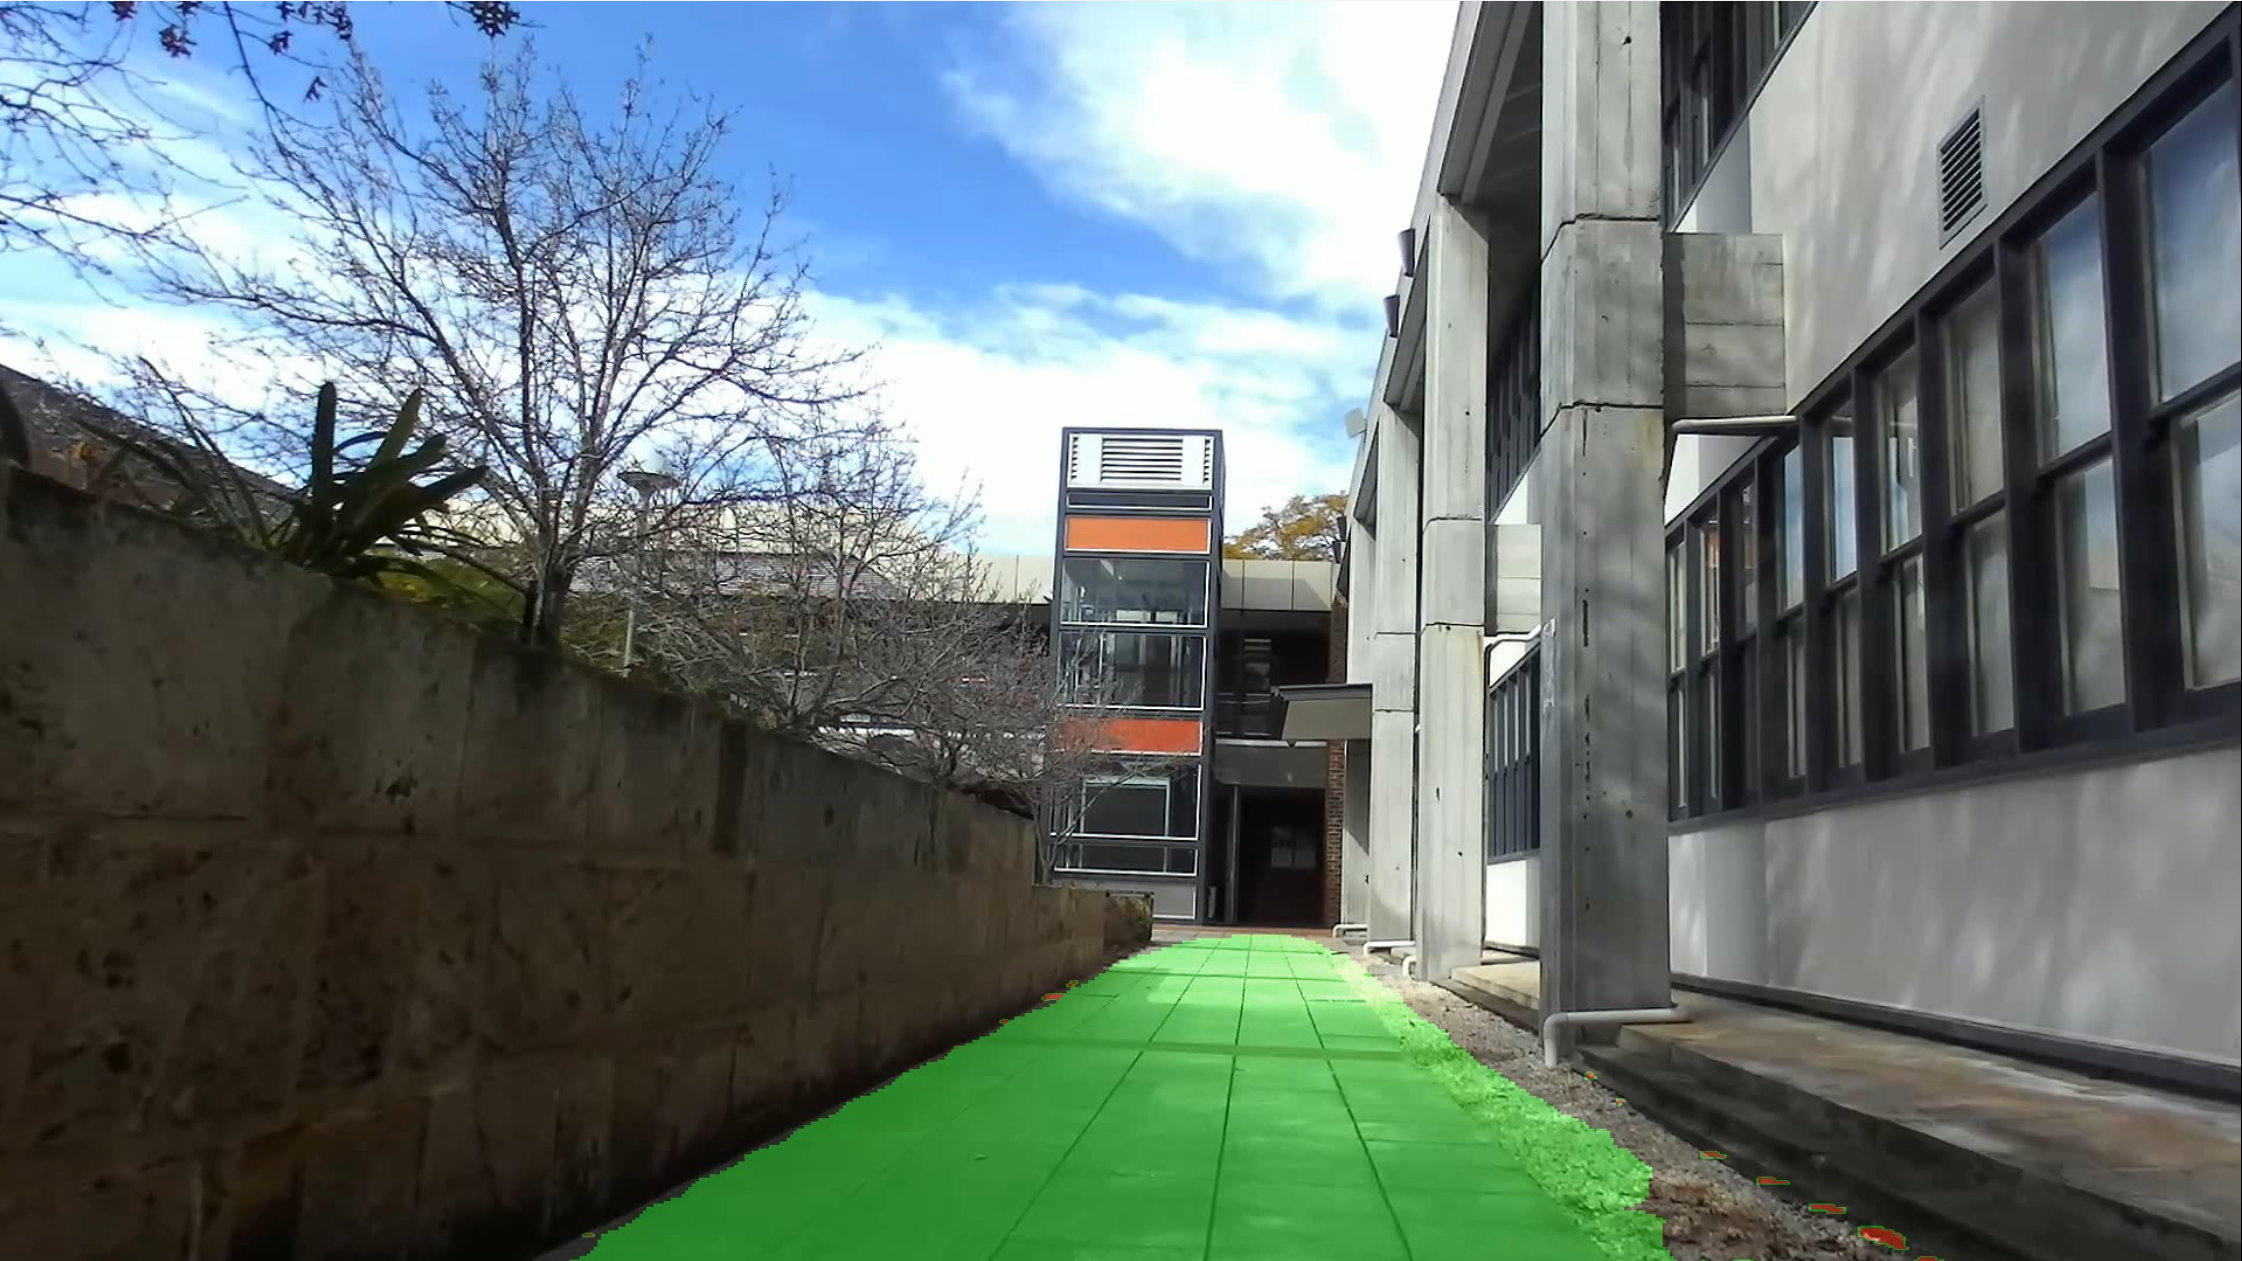
\includegraphics[width=\linewidth]{images/segmentation_3.PNG}
    \end{subfigure}
    \quad
    \begin{subfigure}{.24\textwidth}
        \centering
        \includegraphics[width=\linewidth]{images/occupancy_map3.png}
    \end{subfigure}
    \caption{Segmented image output and corresponding occupancy map for three locations around Curtin university}
    \label{fig:occupancy_map_seg}
\end{figure}

This segmented image to occupancy map transform works well in all observed cases, as long as the Hybridnets model identifies the
drivable area accurately. One improvement that could be made to this implementation is its speed.
The algorithm is bottlenecked by the occupancy map transform code, which takes between \SI{150}{\milli\second}
and \SI{500}{\milli\second} to execute, depending on the size of the drivable area.

Although this approach reliably maps drivable areas to an occupancy grid,
the area directly in front of the wheelchair (approx. \SI{2.6}{\metre}) and behind the wheelchair is unknown due to the FOV of the camera.
Several approaches to rectify this are explored in \cref{sec:future_work}.

A comparison of the occupancy map before and after morphological processing is shown in \cref{fig:morphological_processing}.
Although the occupancy map has a higher resolution before this transformation, the poor density of the map
could make it more difficult to process. The time taken to perform this morphological processing is negligible
when compared to other sections of this code.

\begin{figure}[b]
    % 16:6 width ratio
    % 0.64, 0.24
    \centering
    \begin{subfigure}{.3\textwidth}
        \centering
        \includegraphics[width=\linewidth]{images/occupancy_map1_nomorph.png}
        \caption{Before processing}
    \end{subfigure}
    \quad
    \begin{subfigure}{.3\textwidth}
        \centering
        \includegraphics[width=\linewidth]{images/occupancy_map1.png}
        \caption{After processing}
    \end{subfigure}
    \caption{Comparison of occupancy map before and after morphological processing}
    \label{fig:morphological_processing}
\end{figure}

\subsection{Evaluation of 3D point cloud obstacle detection algorithms}
% sensor tilt, find_floor_plane
% compare performance vs ultra depth mode
Direct processing of the 3D point cloud data was tested to identify environmental obstacles and drivable areas.
One such approach involved using the inbuilt ZED SDK function \texttt{find\_floor\_plane},
which outputs a polygon of the floor plane.
This is shown in \cref{fig:find_floor_plane} and compared alongside the segmentation occupancy map.
This approach is very poor at identifying the floor plane accurately and has large frame-to-frame
variation in its output. The only redeeming factor of this approach is its speed;
as the function is GPU accelerated, this calculation takes approximately \SI{60}{\milli\second}.

\begin{figure}[b]
    % 16:6 width ratio
    % 0.64, 0.24
    \centering
    \begin{subfigure}{.5\textwidth}
        \centering
        \includegraphics[width=\linewidth]{images/find_floor_plane_video.PNG}
        \caption{Video footage}
    \end{subfigure}
    \quad
    \begin{subfigure}{.2\textwidth}
        \centering
        \includegraphics[width=\linewidth]{images/find_floor_plane_seg.PNG}
        \caption{Segmentation occupancy map}
    \end{subfigure}
    \quad
    \begin{subfigure}{.2\textwidth}
        \centering
        \includegraphics[width=\linewidth]{images/find_floor_plane.PNG}
        \caption{Output from \texttt{find\_floor\_plane}}
    \end{subfigure}
    \caption{ZED SDK \texttt{find\_floor\_plane} function compared with segmentation occupancy map}
    \label{fig:find_floor_plane}
\end{figure}

Another approach that was tested was a custom algorithm to process the point cloud data,
detailed in \cref{sec:point_cloud_obstacle_detection}. The results of this algorithm
are shown in three scenarios: one indoor (\cref{fig:pcloud_indoor}) and two outdoor (\cref{fig:pcloud_outdoor_bad} and \cref{fig:pcloud_outdoor_good}).
Note that the drivable area is labelled in green and the environmental obstacles are labelled in red.

\begin{figure}[H]
    % 16:6 width ratio
    % 0.64, 0.24
    \centering
    \begin{subfigure}{.64\textwidth}
        \centering
        \includegraphics[width=\linewidth]{images/pcloud_indoor_video.PNG}
        \caption{Video footage}
    \end{subfigure}
    \quad
    \begin{subfigure}{.24\textwidth}
        \centering
        \includegraphics[width=\linewidth]{images/pcloud_indoor.PNG}
        \caption{Occupancy map}
    \end{subfigure}
    \caption{Point cloud processing result (Indoor)}
    \label{fig:pcloud_indoor}
\end{figure}

\begin{figure}[b]
    % 16:6 width ratio
    % 0.64, 0.24
    \centering
    \begin{subfigure}{.64\textwidth}
        \centering
        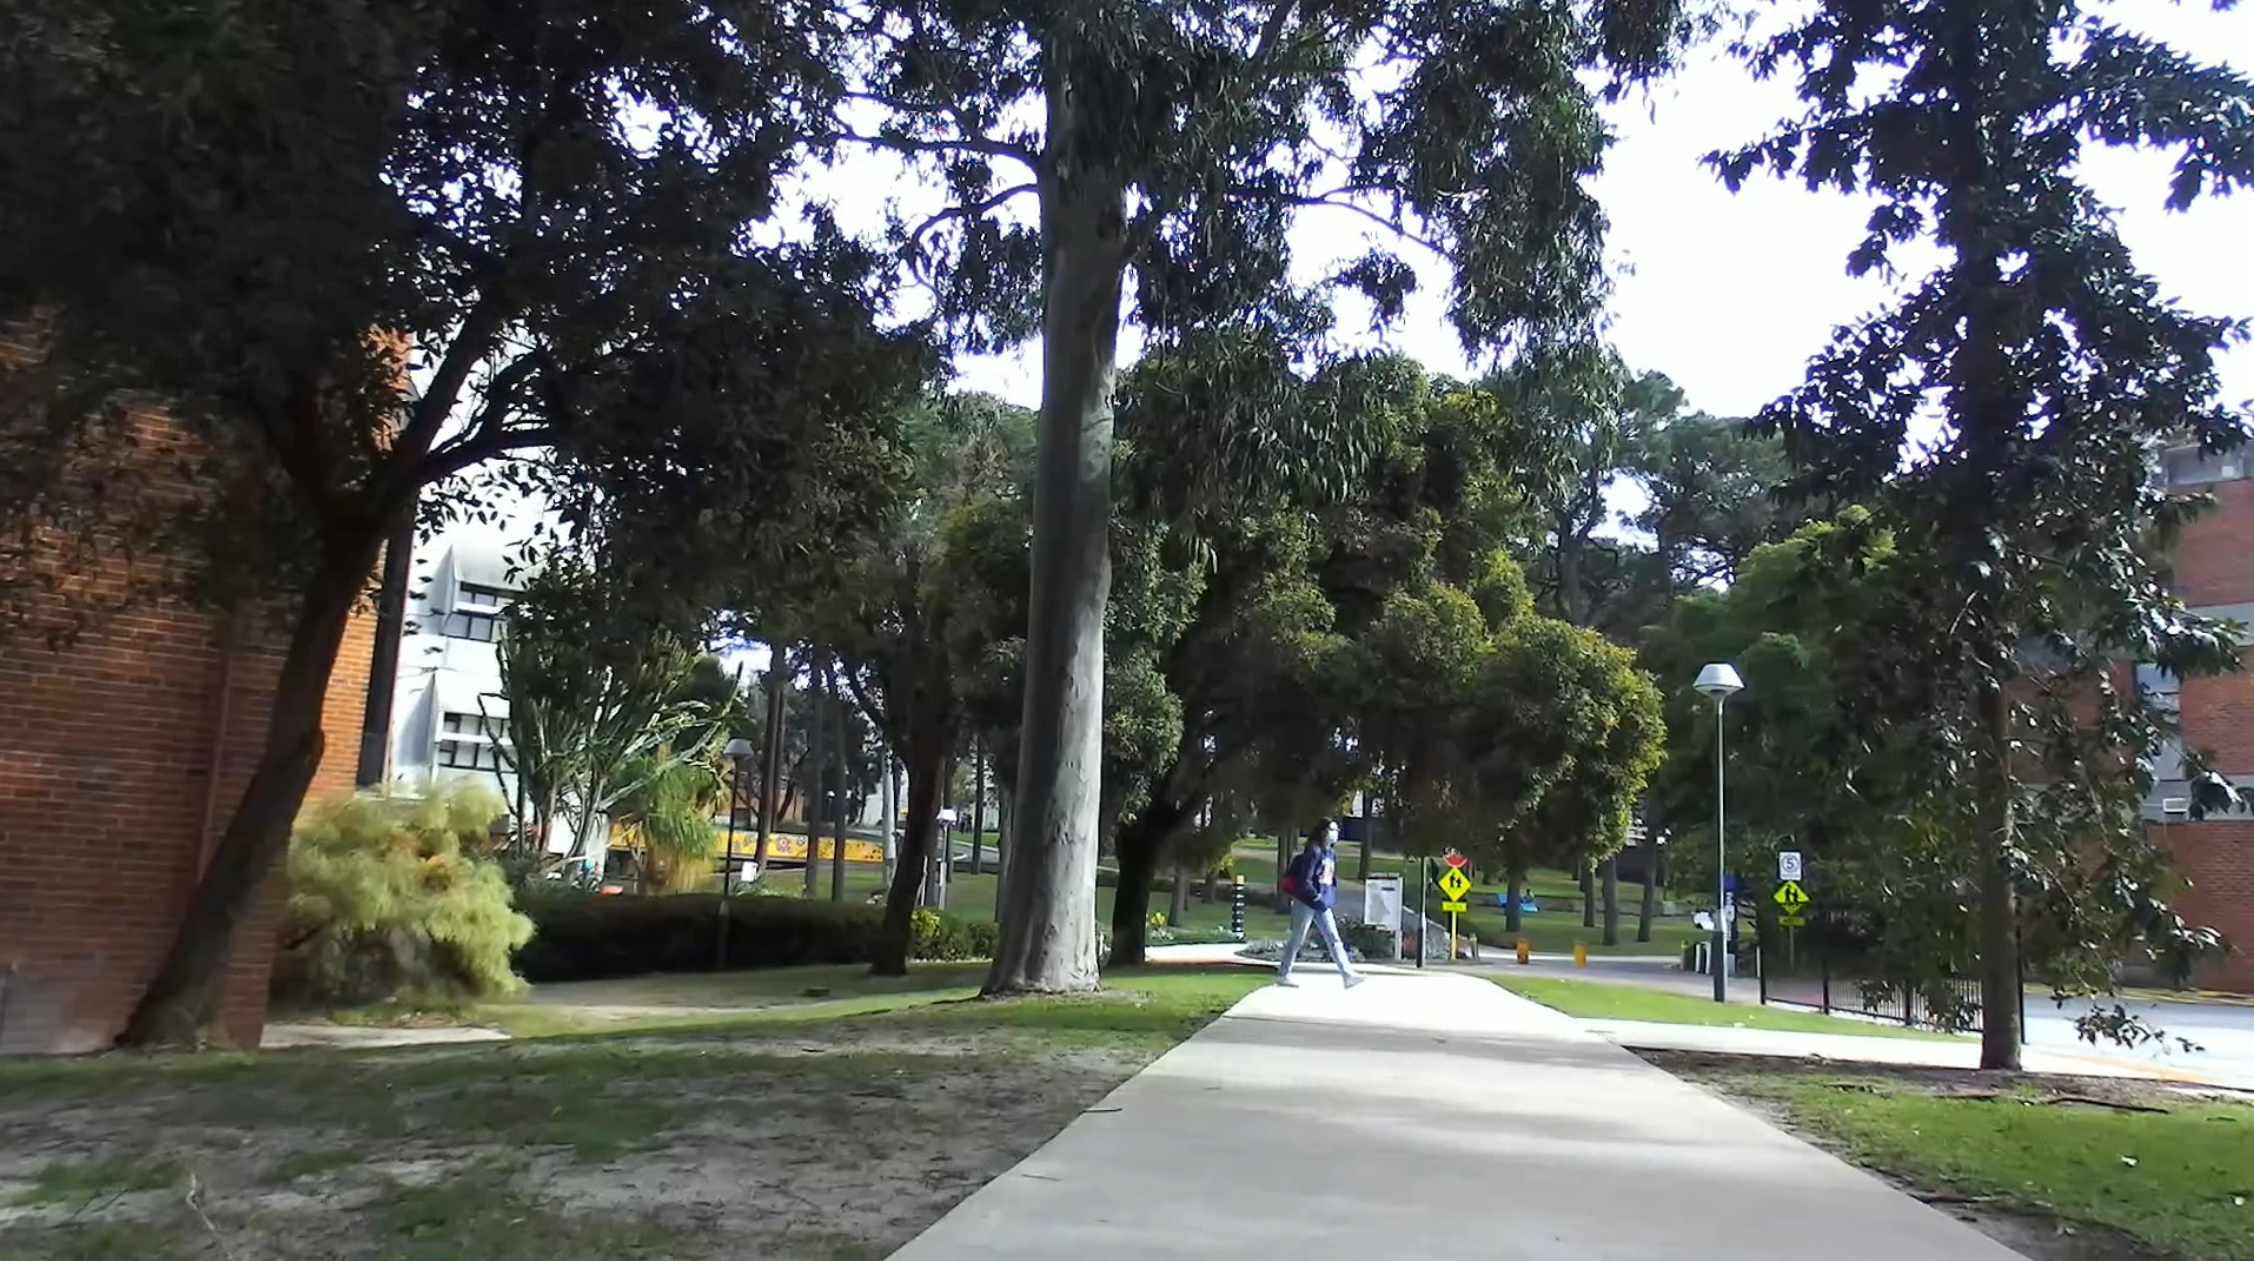
\includegraphics[width=\linewidth]{images/pcloud_outdoor_bad_video.PNG}
        \caption{Video footage}
    \end{subfigure}
    \quad
    \begin{subfigure}{.24\textwidth}
        \centering
        \includegraphics[width=\linewidth]{images/pcloud_outdoor_bad.PNG}
        \caption{Occupancy map}
    \end{subfigure}
    \caption{Point cloud processing result (Outdoor, uniform path)}
    \label{fig:pcloud_outdoor_bad}
\end{figure}

\begin{figure}[b]
    % 16:6 width ratio
    % 0.64, 0.24
    \centering
    \begin{subfigure}{.64\textwidth}
        \centering
        \includegraphics[width=\linewidth]{images/pcloud_outdoor_good_video.PNG}
        \caption{Video footage}
    \end{subfigure}
    \quad
    \begin{subfigure}{.24\textwidth}
        \centering
        \includegraphics[width=\linewidth]{images/pcloud_outdoor_good.PNG}
        \caption{Occupancy map}
    \end{subfigure}
    \caption{Point cloud processing result (Outdoor, wheelchair ramp)}
    \label{fig:pcloud_outdoor_good}
\end{figure}

This algorithm works well in indoor settings (\cref{fig:pcloud_indoor}) at identifying the drivable area
as well as the position of walls and other static objects. Accurate occupancy maps are also generated for
outdoor settings with well-defined boundaries, such as a wheelchair ramp with handrails (\cref{fig:pcloud_outdoor_good}).
However, this algorithm can struggle with open outdoor settings as seen in \cref{fig:pcloud_outdoor_bad}.
Due to the uniformity of the pedestrian path in this image, the ZED Mini is unable to
reliably generate a depth map and 3D point cloud for the path. This leads to the algorithm
mistakenly identifying grassy and uneven terrain as drivable, but not identifying the
path as drivable.

This algorithm is slower than the segmentation approach, with a mean latency of \SI{550}{\milli\second}.
Due to this limitation, it is more suited for identifying non-moving objects such as walls
as opposed to identifying moving objects such as people and vehicles.

The ZED Mini has three depth modes: \texttt{ULTRA}, \texttt{QUALITY}, and \texttt{PERFORMANCE}.
These depth modes trade performance for depth accuracy - a comparison between the occupancy maps
generated by these modes can be seen in \cref{fig:depth_mode_comparison}.
The \texttt{ULTRA} depth mode accurately identifies the back wall as flat.
However, the \texttt{PERFORMANCE} depth mode does not identify the back wall
as flat, and incorrectly classifies an area beyond the wall as drivable.
Due to the high latency of the rest of this algorithm, the difference in speed between these two depth modes is negligible,
and therefore the \texttt{ULTRA} depth mode was selected.

%% can include some ramp comparisons if need be, but probably not

\begin{figure}[b]
    % 16:6 width ratio
    % 0.64, 0.24
    \centering
    \begin{subfigure}{.5\textwidth}
        \centering
        \includegraphics[width=\linewidth]{images/pcloud_indoor_comparison.PNG}
        \caption{Video footage}
    \end{subfigure}
    \quad
    \begin{subfigure}{.2\textwidth}
        \centering
        \includegraphics[width=\linewidth]{images/pcloud_indoor_performance.PNG}
        \caption{Performance depth mode}
    \end{subfigure}
    \begin{subfigure}{.2\textwidth}
        \centering
        \includegraphics[width=\linewidth]{images/pcloud_indoor_ultra.PNG}
        \caption{Ultra depth mode}
    \end{subfigure}
    \caption{Comparison of ZED Mini depth modes}
    \label{fig:depth_mode_comparison}
\end{figure}

\subsection{Evaluation of assistive control algorithm}
VFH+ was implemented as a proof-of-concept assistive control algorithm.
This algorithm blends the user's target direction with the occupancy map
to determine a safe steering direction.

\Cref{fig:vfh_implementation} shows the VFH+ algorithm detecting an obstacle in front of
the wheelchair and steering left to avoid this obstacle. This
%demonstrates that  VFH+ works reliably as an assistive control algorithm and
showcases the end-to-end navigation assistance pipeline,
from environmental obstacle detection to
avoidance of that obstacle using VFH+.

The VFH+ algorithm takes
\SI{240}{\milli\second} to determine the steering direction, which increases to
\SI{430}{\milli\second} when called from Python due to the overhead of the MATLAB Engine API.
This latency could be a concern for a complete semi-autonomous wheelchair implementation;
however, this algorithm is a proof of concept, and latency was not a concern during implementation.
Additionally, VFH+ only adjusts the direction of the wheelchair and not the wheelchair's speed,
making it unsuitable as a final assistive control algorithm.

Due to the FOV of the camera, obstacles directly to the left or right of the wheelchair are not added
to the occupancy map. \Cref{fig:vfh_mistake} demonstrates a scenario where this can
become an issue. VFH+ mistakenly steers to the left to avoid the narrow hallway walls,
which would cause a crash with the walls directly to the left of the wheelchair.
This occurs because these walls are not in the occupancy map, and so the VFH+ algorithm
assumes that there is free space in this area.
Several approaches that could improve the occupancy map and rectify this issue
are suggested in \cref{sec:future_work}.

\begin{figure}[b]
    % 16:6 width ratio
    % 0.64, 0.24
    \centering
    \begin{subfigure}{.6\textwidth}
        \centering
        \includegraphics[width=\linewidth]{images/vfh_example_video.PNG}
        \caption{Video footage}
    \end{subfigure}
    \quad
    \begin{subfigure}{.3\textwidth}
        \centering
        \includegraphics[width=\linewidth]{images/vfh_example_map.PNG}
        \caption{Occupancy map}
    \end{subfigure}
    \begin{subfigure}{.45\textwidth}
        \centering
        \includegraphics[width=\linewidth]{images/vfh_example_lidar.PNG}
        \caption{Binary occupancy grid and LIDAR scan of obstacles}
    \end{subfigure}
    \quad
    \begin{subfigure}{.45\textwidth}
        \centering
        \includegraphics[width=\linewidth]{images/vfh_example_hist.PNG}
        \caption{Polar histogram of obstacles with target and steering directions}
    \end{subfigure}
    \caption{VFH+ changing direction to avoid an obstacle}
    \label{fig:vfh_implementation}
\end{figure}

\begin{figure}[b]
    % 16:6 width ratio
    % 0.64, 0.24
    \centering
    \begin{subfigure}{.6\textwidth}
        \centering
        \includegraphics[width=\linewidth]{images/vfh_fov_video.PNG}
        \caption{Video footage}
    \end{subfigure}
    \quad
    \begin{subfigure}{.3\textwidth}
        \centering
        \includegraphics[width=\linewidth]{images/vfh_fov_map.PNG}
        \caption{Occupancy map}
    \end{subfigure}
    \begin{subfigure}{.45\textwidth}
        \centering
        \includegraphics[width=\linewidth]{images/vfh_fov_lidar.PNG}
        \caption{Binary occupancy grid and LIDAR scan of obstacles}
    \end{subfigure}
    \quad
    \begin{subfigure}{.45\textwidth}
        \centering
        \includegraphics[width=\linewidth]{images/vfh_fov_hist.PNG}
        \caption{Polar histogram of obstacles with target and steering directions}
    \end{subfigure}
    \caption{VFH+ mistakenly changing direction due to low sensor FOV}
    \label{fig:vfh_mistake}
\end{figure}

% include speed, turning behind

\subsection{Evaluation of pose estimation APIs}
% positional tracking API
